% Options for packages loaded elsewhere
\PassOptionsToPackage{unicode}{hyperref}
\PassOptionsToPackage{hyphens}{url}
%
\documentclass[
  11pt,
  b5paper,
]{article}
\usepackage{lmodern}
\usepackage{amssymb,amsmath}
\usepackage{ifxetex,ifluatex}
\ifnum 0\ifxetex 1\fi\ifluatex 1\fi=0 % if pdftex
  \usepackage[T1]{fontenc}
  \usepackage[utf8]{inputenc}
  \usepackage{textcomp} % provide euro and other symbols
\else % if luatex or xetex
  \usepackage{unicode-math}
  \defaultfontfeatures{Scale=MatchLowercase}
  \defaultfontfeatures[\rmfamily]{Ligatures=TeX,Scale=1}
  \setmainfont[]{Times New Roman}
\fi
% Use upquote if available, for straight quotes in verbatim environments
\IfFileExists{upquote.sty}{\usepackage{upquote}}{}
\IfFileExists{microtype.sty}{% use microtype if available
  \usepackage[]{microtype}
  \UseMicrotypeSet[protrusion]{basicmath} % disable protrusion for tt fonts
}{}
\makeatletter
\@ifundefined{KOMAClassName}{% if non-KOMA class
  \IfFileExists{parskip.sty}{%
    \usepackage{parskip}
  }{% else
    \setlength{\parindent}{0pt}
    \setlength{\parskip}{6pt plus 2pt minus 1pt}}
}{% if KOMA class
  \KOMAoptions{parskip=half}}
\makeatother
\usepackage{xcolor}
\IfFileExists{xurl.sty}{\usepackage{xurl}}{} % add URL line breaks if available
\IfFileExists{bookmark.sty}{\usepackage{bookmark}}{\usepackage{hyperref}}
\hypersetup{
  pdftitle={An analysis of tone implementation in a Gbe language using forced alignment},
  hidelinks,
  pdfcreator={LaTeX via pandoc}}
\urlstyle{same} % disable monospaced font for URLs
\usepackage[margin=2.5cm]{geometry}
\usepackage{graphicx}
\makeatletter
\def\maxwidth{\ifdim\Gin@nat@width>\linewidth\linewidth\else\Gin@nat@width\fi}
\def\maxheight{\ifdim\Gin@nat@height>\textheight\textheight\else\Gin@nat@height\fi}
\makeatother
% Scale images if necessary, so that they will not overflow the page
% margins by default, and it is still possible to overwrite the defaults
% using explicit options in \includegraphics[width, height, ...]{}
\setkeys{Gin}{width=\maxwidth,height=\maxheight,keepaspectratio}
% Set default figure placement to htbp
\makeatletter
\def\fps@figure{htbp}
\makeatother
\setlength{\emergencystretch}{3em} % prevent overfull lines
\providecommand{\tightlist}{%
  \setlength{\itemsep}{0pt}\setlength{\parskip}{0pt}}
\setcounter{secnumdepth}{3}
\usepackage{linguex}
\usepackage[style=authoryear,]{biblatex}
\addbibresource{localbibliography.bib}

\title{An analysis of tone implementation in a Gbe language using forced
alignment}
\author{}
\date{}

\begin{document}
\maketitle

\hypertarget{abstract}{%
\section*{Abstract}\label{abstract}}
\addcontentsline{toc}{section}{Abstract}

This study applies forced alignment tools to an acoustic corpus of nine
texts from a Saxwe {[}sxw{]} (Gbe) speaker in order to investigate the
phonetic implementation of: 1) tone spread, 2) non-automatic downstep,
and 3) intonational phrase (IP) boundary tones. Using this methodology,
we find quantitative evidence of rightward spread of underlying high (H)
and low (L) to a toneless (Ø) tone-bearing unit. We also identify
non-automatic downstep as having a median F0 fall of 2 semitones, which
is a statistically significant difference from the greater F0 fall from
H to L.

We then consider the tonal effects of IP boundaries and find that there
is evidence of pitch resetting at IP boundaries which are
utterance-medial. Comparing adjacent vowels of identical lexical tone,
this corresponds to a median F0 fall of 2.5 semitones before the
boundary and a median F0 rise of 2 semitones crossing the boundary.
Narrowing our examination to looking within the pre-boundary vowel, we
see that there is accomodation between lexical and boundary tone, as
evidenced by a lowering of pitch realization for H tone observable
within the vowel which immediately precedes an utterance-medial L\% IP
boundary. However, if we look at an IP boundary which is
utterance-final, there is no lowering of the pitch trajectory of H. A
further observation seen in all pitch trajectories is that lexical L,
whether adjacent to a boundary or not, is always realized with a falling
pitch trajectory across the duration of the vowel; the rate of decrease
in F0 varies depending on the environment.

Finally, we discuss the limitations and advantages of using automated
alignment tools and corpus data for tone analysis in African languages.

\hypertarget{background}{%
\section{Background}\label{background}}

\hypertarget{corpus-level-study-of-the-phonetic-implementation-of-tone}{%
\subsection{Corpus-level study of the phonetic implementation of
tone}\label{corpus-level-study-of-the-phonetic-implementation-of-tone}}

Research into the phonetic interpretation of tone is often based on
studies of elicited data at the utterance level rather than text-level
unprepared speech. This is in part due to the time-consuming process of
identifying in acoustic data the boundaries of all of the tone-bearing
sounds (typically vowels) in natural speech prior to taking F0
measurements. However, with the rise of corpus phonetics which involves
the ``large-scale quantitative analysis of acoustic corpus data''
\autocite{yao_automated_2010}, new insights can be obtained from larger
collections of texts and transcriptions
\autocite{chodroff_structured_2015}. Corpus phonetics has started to be
applied to under-documented languages \autocite{kempton_corpus_2020} but
there can be a tension between the large-scale ambitions for corpus
phonetics and the reality of the small quantity of data available in
lower resource languages. This study is based on a corpus of nine texts
which includes 1773 vowels. The corpus was produced by a single speaker
of Saxwe {[}sxw{]}, a language of the Gbe continuum
\autocite{capo_elements_1984,Capo1991comparative} spoken in the country
of Benin \autocite{eberhard_ethnologue_2019}. In this study, we
investigate several research questions related to the phonetic
implementation of tone and we evaluate the strengths and weaknesses of
using a corpus-based approach to doing tone research.

The overall approach to studying tone implementation is as follows.
Forced alignment speech recognition tools are used to align phone
transcripts to audio files, thus allowing for the automated measurement
of F0 values of all the vowels found in this text corpus. Following
this, these measurements of F0 values are then associated with
information obtained from previous studies about the underlying lexical
identity --- high (H), low (L), or toneless (Ø) --- of each of the
vowels in the database used.

Based on this information, we investigate three research questions
formulated as follows. First, what is the phonetic implementation of
underlying lexical tone in processes of tonal spread? Second, what is
the impact on F0 when there is non-automatic downstep? Third, what is
the effect of intonational phrase boundaries on pitch? In answering this
latter question, we look at both utterance-medial and utterance-final
boundaries.

\hypertarget{tone-lowering-trends-and-the-tonal-effect-of-phonological-boundaries}{%
\subsection{Tone lowering trends and the tonal effect of phonological
boundaries}\label{tone-lowering-trends-and-the-tonal-effect-of-phonological-boundaries}}

There are several pitch lowering trends related to H tone production,
with some important differences between them
\autocite{connell_downstep_2011,Downing2017Introduction,Gussenhoven2004phonology}.
One of the primary distinctions made is between automatic and
non-automatic downstep. Automatic downstep (also known as ``downdrift'')
is triggered by a surface L between Hs, while non-automatic downstep
(also known simply as ``downstep'') is often triggered by either a
floating L between Hs or by adjacent Hs on the tonal tier --- a
violation of the Obligatory Contour Principle. Downstep of either type
is sometimes described as a change in register because the lowering
produces a new ``ceiling'' for the production of H tone such that H will
no longer be realized above this lowered F0 measurement
\autocite{Clements1979description,connell_downstep_2011}.

Assuming a \{H, Ø, L\} inventory\footnote{The inventory we adopt here
  differs from the \{H, M, L\} interpretation adopted in
  \textcite{Beavon-Ham2019Tone} (where `M' represents mid tone).} of
underlying tones in Saxwe, non-automatic downstep is triggered primarily
as a result of the rightward iterative spread of H tone to adjacent
toneless vowels until a new lexical H tone is reached---thus creating a
violation of the Obligatory Contour Principle and the phonetic lowering
of pitch which is an effect of this \autocite[241--245,
264--282]{Beavon-Ham2019Tone}. Although floating L tones may also be a
trigger of non-automatic downstep, these cases of downstep are not
addressed in this study. The utterance-level F0 data presented in
\textcite{Beavon-Ham2019Tone} support the claim that non-automatic
downstep is a part of the phonetic implementation of Saxwe; this study
examines that implementation within an unelicited corpus.

Declination is the gradual (as opposed to punctual) lowering of F0
unrelated to any phonological influence
\autocite{connell_downstep_2011,Downing2017Introduction}. It can be
difficult to obtain measurements for declination apart from observing
the trends of sequences of identical tones. One of the challenges in
discussions of downstep is to discern the difference between the
lowering due to declination and the lowering due specifically to either
automatic or non-automatic downstep.

Another lowering trend is final lowering. In final lowering, the F0 on
the final syllable of a tonal domain can sometimes be lowered
\autocite{Herman1996Final,pierrehumbert_japanese_1988}. It is not always
clear in the literature whether final lowering is considered
attributable to an interaction with a tonal boundary or not. This leads
us then to a discussion of the effect of phonological boundaries on tone
implementation.

While a variety of levels of phonological boundary effects may be
studied (from word to intonational phrase-level), this study focuses on
the tonal effect of intonational phrase (IP) boundaries. Intonational
boundary tone, if it exists in a given language, can interact with
lexical tones in several ways
\autocite{Downing2017Introduction,hyman_tonal_2011,downing_intonation_2017-1}.
According to \textcite{hyman_tonal_2011}, the phonetic implementation
may demonstrate what they label as ``accommodation'', where the F0
patterns include observations attributable to both the lexical tone and
the intonational boundary tone. This may be observed solely on the final
syllable of the utterance or it may be observed over multiple syllables
in the utterance. Other possibilities for interaction are that the
lexical tone is neutralized in the presence of an intonational boundary
tone (labeled as ``submission'') or, conversely, that lexical tone
avoids all influence due to intonational boundary tone (labeled as
``avoidance'').

IP boundaries may coincide with several syntactic structures. The
clearest division that can be made between IP boundaries is the division
between utterance-medial IP boundaries and utterance-final IP
boundaries. We further subdivide utterance-medial IP boundaries into: 1)
those associated with fronted constituents and, 2) those associated with
post-clause constituents. In the first group, the boundary precedes the
subject of the main clause. This group includes cases of topic
structures (where a resumptive pronoun is found in the main clause) as
well as phrases and dependent clauses that precede the main clause. For
the second group (IP boundaries associated with post-clause
constituents), the boundary occurs to the right of the main or
independent clause. This includes cases of coordinate clauses,
consecutive clauses, and dependent clauses that follow the main clause.

The assumption in this study is that IP boundaries do not necessarily
coincide with every instance of a particular syntactic structure. For
example, coordinate clauses may have an IP boundary between the two
clauses or they may be realized as a single IP. The decision to signal
the existence of an IP boundary was based on a perception of there being
a pause in the stream of speech, sometimes preceded by a lengthening of
the duration of the immediately preceding syllable. Utterance-final
boundaries were also signaled by a pause, sometimes with an audible
breath intake in the stream of speech. Unfinished utterances were not
signaled as having an utterance-final IP boundary. The following
examples provide illustrations of the IP boundaries for fronted
constituents, post-clause constituents, and utterances.\footnote{The
  following abbreviations are used in these examples: 3 (third person),
  COMPL (completive), CONJ (conjunction), DET (determiner), FUT
  (future), INDEF (indefinite determiner), PL (plural), SG (singular),
  SS (same subject).}

In examples \ref{ex:fc1} and \ref{ex:fc2}, we see a fronted constituent
composed of a subordinate clause. The IP boundary is located at the end
of this clause, marked as \%. There is also an IP boundary at the end of
the utterance. As seen in Figure \ref{fig:fc1}, there is a brief pause
at the boundary of the embedded IP of the fronted constituent.

\exg. \label{ex:fc1}/nã́ aji lá sjɛ̃́ vɔ̀ je nã và ji gbɛ̃̀/\\
when bean DET harden COMPL they FUT come go pick:3SG\\
When the beans harden, they will pick them. (Texts, T0003)

\ex. \label{ex:fc2}((nã aji la sjɛ̃ vɔ \%)ɩ je nã va ji gbɛ̃ \%)ɩ

\begin{figure}
\centering
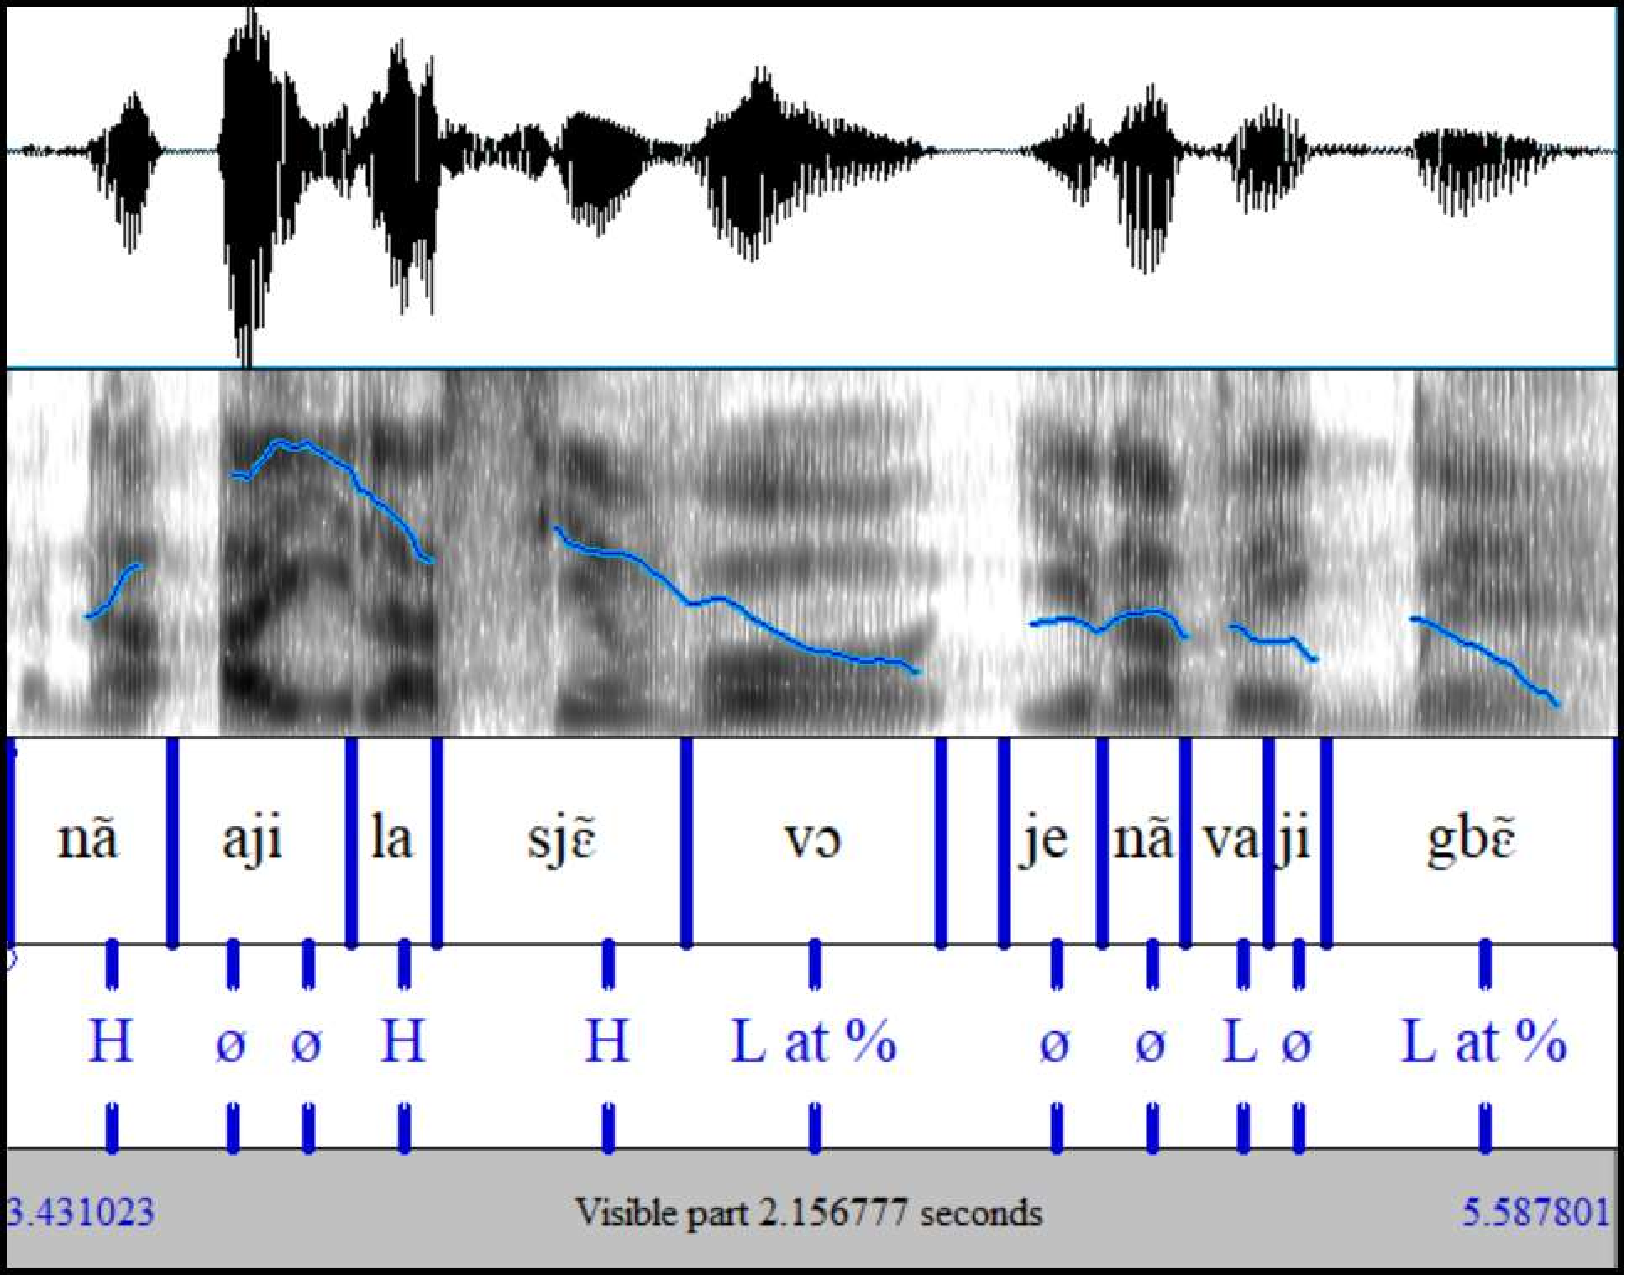
\includegraphics[width=0.75\textwidth,height=0.75\textheight]{figure/fronted-constituent-boundary.pdf}
\caption{Waveform, spectrogram and pitch trace in Praat of example
\ref{ex:fc1} showing a fronted constituent.\label{fig:fc1}}
\end{figure}

In examples \ref{ex:pc1} and \ref{ex:pc2}, we again see a fronted
constituent composed of a subordinate clause, its boundary marked with
\%. In addition, we see two independent clauses in a relation of
coordination. Between these two, there is an IP boundary, marked with
the second instance of the \% symbol. This is an example of what we
label in this study as a post-clause constituent. Figure \ref{fig:pc1}
shows a pause between the two IPs at this post-clause boundary. Finally,
there is an utterance-final IP boundary.

\exg. \label{ex:pc1}/je gbɛ̃̀ vɔ̀ je nã và ji sɔ́ kɔ̃ dò fí ɖé á bo xwjá-ɛ
{[}xwjɛ{]}/\\
3PL pick:3SG COMPL 3PL FUT come go take pile at place INDEF CONJ CONJ:SS
dry:3SG\\
When they have picked it, they take and pile it somewhere and dry it.
(Texts, T0003)

\ex. \label{ex:pc2}(((je gbɛ̃ vɔ \%)ɩ je nã va ji sɔ kɔ̃ dò fi ɖe \%)ɩ (a
bo xwjɛ)\%)ɩ

\begin{figure}
\centering
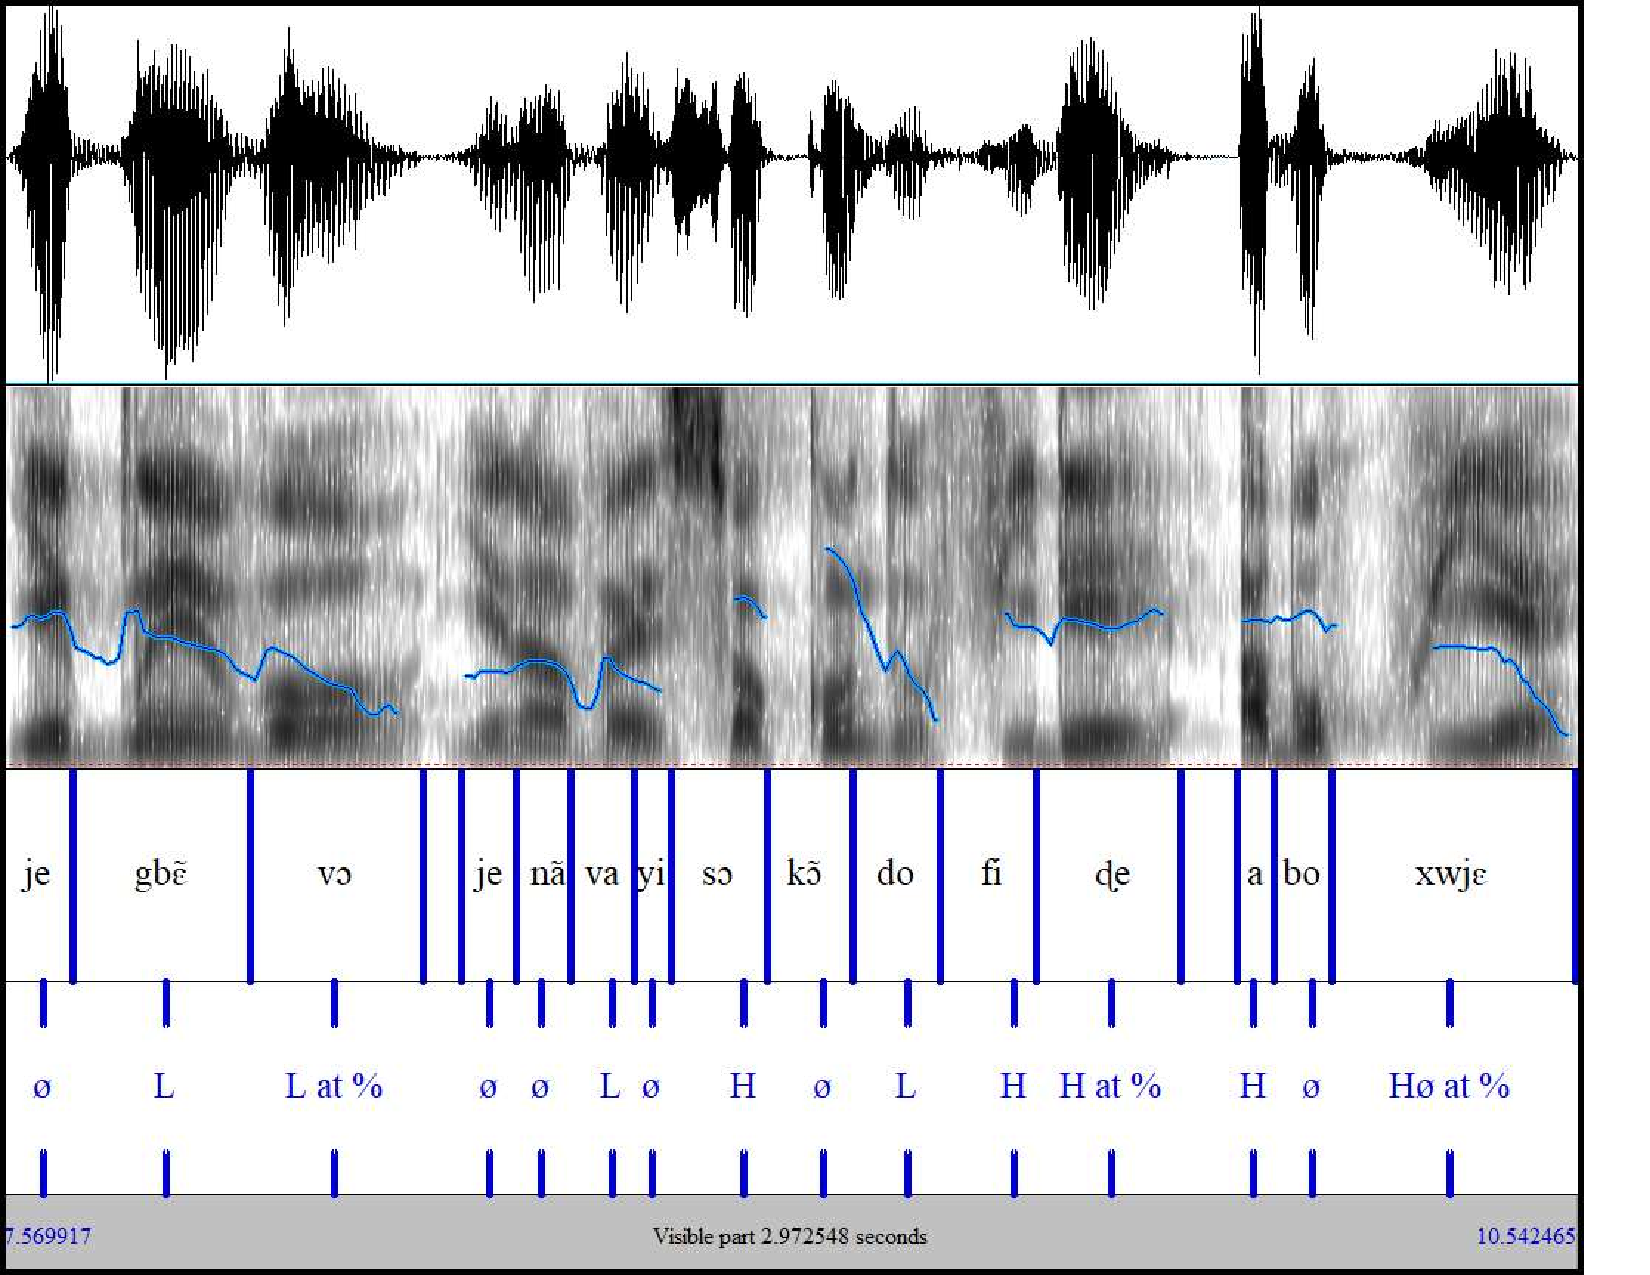
\includegraphics[width=0.75\textwidth,height=0.75\textheight]{figure/post-clause-boundary.pdf}
\caption{Waveform, spectrogram and pitch trace in Praat of example
\ref{ex:pc1} showing a post-clause constituent).\label{fig:pc1}}
\end{figure}

Note that there is no IP boundary between the verbs /sɔ/ `take' and /kɔ̃
/ `pile' in the serial verb construction in example \ref{ex:pc1}. There
is no pause between the two, nor is there a lengthening in the stream of
speech in the articulation of these two verbs one after the other.

\hypertarget{experimental-set-up}{%
\section{Experimental set-up}\label{experimental-set-up}}

The acoustic recordings used for this study are located in a repository
of Saxwe data.\footnote{\url{https://drive.google.com/open?id=10LDp4U5snDEMBlXbSvZKiq-YHvivjvaS}}
These texts were produced by André Taïve, a man in his early 40s at the
time when the texts were recorded in 2015. Recordings were done on a
Marantz PMD 660 solid state recorder using an external Shure SM10A
headworn, unidirectional dynamic microphone. Transcripts of the texts
were done in consultation with the speaker. The nine texts in this
corpus amounted to just under 7 minutes of acoustic data composed of 84
utterances containing 1773 vowels.

The workflow for the alignment process involved a number of software
tools. First, SayMore \autocite{sil_international_saymore_2019} was used
as a platform to segment the audio recordings into utterances and to
create the phonetic transcriptions. ELAN \autocite{elan_elan_2019} was
then used to convert these transcriptions into a suitable format for
alignment (Praat Textgrids). Montreal Forced Aligner
\autocite{mcauliffe_montreal_2018} was used to automatically align these
transcriptions with the audio.

In testing the validity of this process, we used Praat
\autocite{boersma_praat_2019} to produce reliable manual alignments to
evaluate the machine alignments. Finally EMU-SDMS
\autocite{winkelmann_emu-sdms:_2017} was then used for the acoustic
phonetic analysis, alongside various tools in the R programming language
\autocite{r_core_team_r_2020,wickham_tidyverse_2017,aphalo_ggpmisc_2022}.

Lexical tone information was provided through consultation of a Saxwe
FLEx lexicon database
\autocite{sil_international_fieldworks_2017,beavon-ham_saxwe_2020} as
well as from diagnostic tests documented in research on Saxwe tonal
phenomena \autocite{Beavon-Ham2019Tone}. For the purposes of this study,
the intent was to study lexical H, L, and toneless (Ø) vowels. The
following notation was used in assigning lexical tone data to vowels: H
(lexical H tone), L (lexical L tone), Ø (toneless), !H (lexical H tone
immediately preceded by a H tone and a non-zero number of toneless
vowels---in that order), \% (intonational phrase boundary), and LH (both
lexical L and lexical H tone on a single vowel). For underlying LH that
had undergone simplification, the L or H tone remaining after
simplification was assigned as the lexical tone.\footnote{In Saxwe
  monomorphemic forms, the rule observed is that LH contours on a vowel
  are simplified to H following a H vowel and L following a L or
  toneless vowel \autocite{Beavon-Ham2019Tone}.}

In order to test the accuracy of the alignments produced by Montreal
Forced Aligner (MFA), four utterances were randomly selected and
independently manually aligned to create 200 reliable boundaries. The
standard approach to calculating alignment errors involves recording the
absolute error, i.e.~the error whether the machine boundary is to the
right or the left of the manually-aligned boundary. The resulting errors
by MFA were calculated to have a median value of 15 ms and a mean value
of 28 ms for each utterance. However, we found that there was a
significant bias to the errors so that the machine boundary was more
likely to be to the right of the manually aligned boundary. The median
of this bias was 12 ms to the right. This might be an artifact of using
a small corpus where there is less diversity of phonetic environments
present for each phone. In this situation it might be difficult for the
machine to determine exactly where the boundaries are in a string of
phones, i.e.~in the iterative training process there may not be enough
data to correct initially placed boundaries. Interestingly in the
experimental setup for the analysis of a different language
\autocite{kempton_corpus_2020} there was a similar bias but to the left
instead.\footnote{\url{https://groups.google.com/g/mfa-users/c/Rv9C5wzecJ8/m/mJ6QYJ43AAAJ},
  or within Google groups search for the phrase ``Adding 10 ms to every
  boundary seems to improve accuracy''.}

Although the observation has been made that the ``shoulder'' or
stabilization of pitch levels is generally observed at a point about
66\% into the duration of the vowel
\autocite[257--299]{Beavon-Ham2019Tone}, in this study, the F0 value for
each vowel was measured at a point 50\% into the duration of the vowel.
This was done to minimize the impact of forced alignment errors.

To verify that forced alignment errors only resulted in a small number
of spurious measurements outside of the vowel boundaries, the 1773
aligned vowels were measured for duration. Of course, these duration
measurements are subject to the forced-alignment errors themselves but
the large number of vowels measured helps to lessen this effect. The
first quartile (shortest duration) was approximately 50 ms, and the
third quartile was approximately 100 ms. Given that the median
forced-alignment error is 15 ms, it is clear that a vast majority of
vowel measurements are too long in duration to be affected by these
errors in most contexts where a significant number of measurements are
being taken. However, in the study of IP boundary tone, we manually
verified and occasionally corrected the automated alignments of vowels
at IP boundaries. This was done because the number of vowels occurring
at an IP boundary is much smaller than the number of vowels occurring in
the corpus in general, and occasional errors would have a greater impact
on results.

In the interest of having reproducible results, this paper is also
available as an executable notebook alongside the acoustic data and
lexical tone assignments.\footnote{\url{https://github.com/speechchemistry/corpus-phonetics}}

\hypertarget{results}{%
\section{Results}\label{results}}

Our first research question looks at the F0 implementation of tonal
spread as the lexical tone of the preceding vowel spreads to an
underlyingly toneless (Ø) vowel. Figure \ref{fig:transition_to_toneless}
shows the three transitions studied; in each of these transitions, the
second vowel is a toneless vowel. The three transitions studied in this
corpus are: 1) the transition from Ø to Ø, 2) the transition from H to
Ø, and 3) the transition from L to Ø. We are particularly interested to
know whether these transitions are realized as an average pitch rise or
as an average pitch fall. We present these pitch changes of F0 as
equally tempered semitones rather than hertz because we wanted a
measurement that was closer to human auditory perception, intuitive, and
easily compared with other speakers.

\begin{figure}
\centering
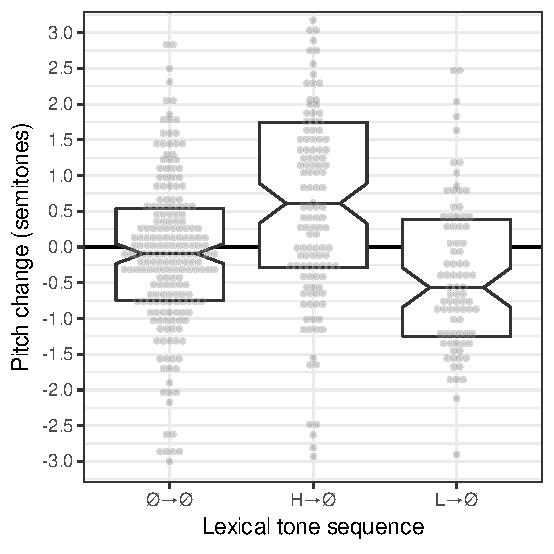
\includegraphics{figure/plot_intervals_of_transitions_to_toneless_syllables-1.pdf}
\caption{Graph showing pitch change for lexical tone transitions to
toneless vowels. (The dot plot has a maximum bin width of 0.1 semitones,
and the box plot notches indicate 95\% confidence intervals for the
population median).\label{fig:transition_to_toneless}}
\end{figure}

In Figure \ref{fig:transition_to_toneless} a dot plot of the intervals
for these three transitions is summarized with a box plot. Each dot
represents a sample; the measurement of a single pitch change from one
vowel to another. Since individual samples are shown as dots there is no
need for box plot whiskers. Alongside the presentation of the sample
median and interquartile range, the box plots also exhibit notches which
indicate the 95\% confidence levels of where the population median lies.
The median pitch changes for these three transitions appear to show: 1)
no pitch change for Ø→Ø, 2) a pitch rise for H→Ø, and 3) a pitch fall
for L→Ø.

There is a large spread of values, and it is important to see if these
pitch changes are statistically significant. A Shapiro-Wilk normality
test of the pitch interval distributions indicated that most of them
were not normally distributed (this was also the case for when pitch
change was measured in hertz). A Wilcoxon single sample signed rank test
was therefore used to test whether the median of each distribution
associated with a transition was different from zero. It was found that
the median pitch change associated with the transition Ø→Ø showed no
statistically significant difference from zero (p = 0.20). However the
median pitch change associated with the other transitions did show a
statistically significant difference from zero: H→Ø (p \textless{}
0.0001), and L→Ø (p = 0.0012). These findings are consistent with the
confidence intervals represented by the box plot notches in Figure
\ref{fig:transition_to_toneless}. These statistical tests alongside all
the other statistical tests in this paper pass corrections for multiple
comparisons (Bonferroni correction).

Our second research question is to examine the interval of pitch change
at the locus of lexical tone transition which is related to
non-automatic downstep; that is, the transition from the last Ø vowel to
!H in an underlying H→Ø\ldots Ø→!H sequence where there are one or
multiple Øs between two lexical Hs and the second H is realized as !H.
By way of comparison, we also look at the transition from H to L, and
the transition from L to H. In Figure \ref{fig:downstep_transition},
intervals of pitch change are again calculated in semitones.

\begin{figure}
\centering
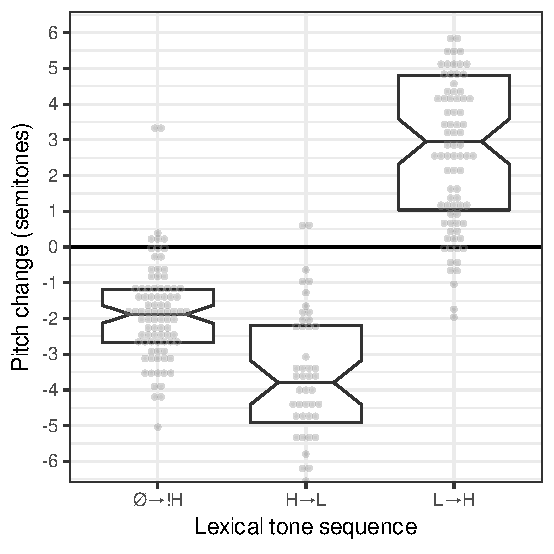
\includegraphics{figure/plot_downstep_transition-1.pdf}
\caption{Graph showing pitch change for lexical tone transitions
relevant to downstep. (The dot plot has a maximum bin width of 0.2
semitones, and the box plot notches indicate 95\% confidence intervals
for the population median).\label{fig:downstep_transition}}
\end{figure}

An initial glance at Figure \ref{fig:downstep_transition} suggests that
the median pitch changes seen in the box plots are approximately: 1) -2
semitones for Ø→!H, 2) -4 semitones for H→L, and 3) +3 semitones for
L→H.

With the spread of values, we wanted to test whether there was a
statistically significant difference for particular pairs of lexical
tone transitions. Using statistical tests we compared Ø→!H and H→L, as
well as H→L and L→H. The Shapiro-Wilk normality test of these pitch
interval distributions indicated that most of them were not normally
distributed. Therefore the non-parametric, Wilcoxon two sample signed
rank test was used to test for differences. When comparing the pitch
intervals for the tone transition Ø→!H and H→L, it was found that there
was a statistically significant difference in the extent of the pitch
fall (p \textless{} 0.0001), with H→L showing a greater pitch fall. In
comparing H→L and L→H it is clear from Figure
\ref{fig:downstep_transition} that there is a difference in the pitch
change but it is interesting to see if the pitch rise is equivalent to
the pitch fall. We found that there was no statistically significant
difference (p=0.068) between the absolute values of the pitch change of
L→H and that of H→L. These findings are all consistent with the box plot
notches.

Our third research question looks at the tonal effects of IP boundaries
associated with three types of grammatical contexts: IP boundaries
associated with fronted constituents, those associated with post-clause
constituents, and those which are utterance-final.

We start by looking at the first two IP boundaries, those associated
with fronted constituents and post-clause constituents. These are both
utterance-medial boundaries. We examine sequences of two vowels with
identical underlying tones (both either H, Ø, or L) in two contexts with
reference to the utterance-medial IP boundary: 1) the context in which
the second vowel is located immediately preceding the IP boundary and
therefore one could describe the two vowels as \emph{before} the IP
boundary, and 2) the context in which the two vowels are located on
either side of the IP boundary and therefore one could describe the two
vowels as \emph{crossing} the IP boundary. We compare these two contexts
with the context where there are adjacent underlying tones with no IP
boundary present.

In this comparison, we measure the difference in F0 realization between
all combined instances of consecutive identical lexical tones which
immediately precede or cross an utterance-medial IP boundary or which
are realized with no IP boundary present; e.g.~for H→H or L→L. By doing
this, we are able to have more statistically significant findings
regarding pitch resetting in this corpus.

\begin{figure}
\centering
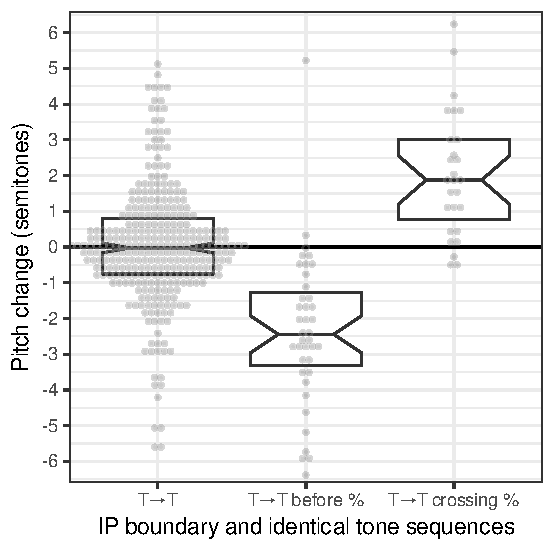
\includegraphics{figure/plot-transitions-1.pdf}
\caption{Graph showing pitch change for sequences with identical lexical
tone as they interact with the utterance-medial IP boundary. This
includes the sequence as it approaches the IP boundary and as it crosses
the IP
boundary.\label{fig:vowel_sequences_and_medial_boundaries_manual}}
\end{figure}

In Figure \ref{fig:vowel_sequences_and_medial_boundaries_manual}, the
median pitch changes for these two contexts appear to show: 1) no
significant difference in pitch between adjacent identical tones in the
absence of a boundary, 2) a median F0 fall of approximately 2.5
semitones for identical tones immediately preceding the IP boundary, and
3) a median F0 rise of approximately 2 semitones for identical tones
crossing the IP boundary.

As in the previous experiments, the Shapiro-Wilk normality test of the
pitch interval distributions indicated that most of them were not
normally distributed. A Wilcoxon single sample signed rank test was
therefore used to test whether the median of each distribution
associated with a transition was different from zero. It was found that
the median pitch change associated with the transition T→T showed no
statistically significant difference from zero (p = 0.86). However the
median pitch change associated with the other transitions did show a
statistically significant difference from zero: T→T before \% (p
\textless{} 0.0001, and T→T crossing \% (p \textless{} 0.0001). These
findings are consistent with the confidence intervals represented by the
box plot notches in Figure
\ref{fig:vowel_sequences_and_medial_boundaries_manual}.

Narrowing our examination to looking specifically at the pre-boundary
vowel, we obtain pitch trajectories for the vowels which immediately
precede an IP boundary and compare these to pitch trajectories for
vowels in the larger corpus where IP boundaries are not present. We seek
to describe how lexical tone and IP boundary tone interact on the final
vowel of an IP. We therefore omit underlyingly toneless vowels from
these pitch trajectories because underlyingly toneless vowels introduce
greater complexity due to tonal spread from a preceding lexical H or L.

\begin{figure}
\centering
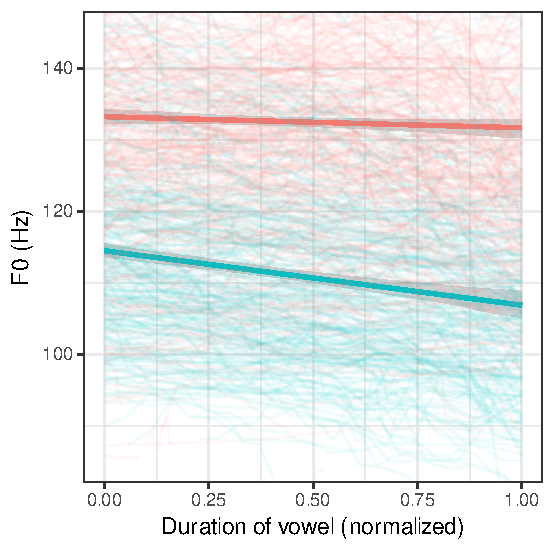
\includegraphics{figure/vowel-pitch-HL-noboundary-manual-1.pdf}
\caption{Pitch trajectories of lexical H (top) and L (bottom) vowels
wherever IP boundaries are absent. Faint lines show individual
trajectories and the solid lines show the median trends. Gray bands show
the 95\% confidence intervals.
\label{fig:vowel_pitch_HL_noboundary_manual}}
\end{figure}

Figure \ref{fig:vowel_pitch_HL_noboundary_manual} gives the pitch
trajectories of lexical H and L vowels in the entirety of our corpus
wherever IP boundaries are absent. This figure shows F0 trajectories on
a single vowel as opposed to the F0 change over a vowel sequence. The
straight solid lines represent the median trends of the trajectories
calculated using linear quantile regression and the gray bands represent
the 95\% confidence intervals. Both median trends are fairly level with
lexical L showing slightly more of a fall; a fall of approximately 8 Hz
over the duration of the vowel.

We turn now to an examination of lexical H and L vowels which precede an
IP boundary correlated with either a fronted constituent or a
post-clause constituent.

\begin{figure}
\centering
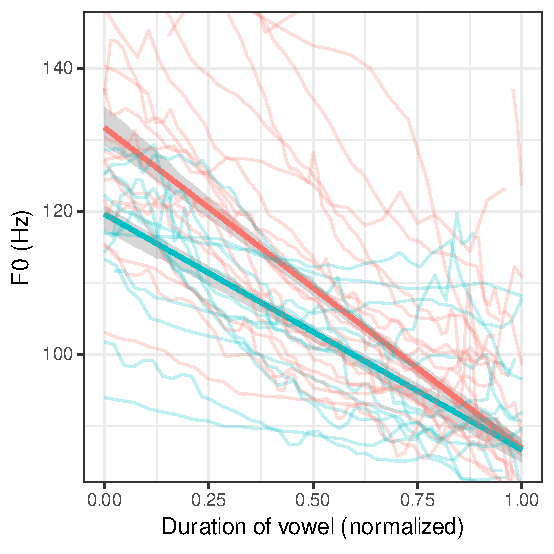
\includegraphics{figure/vowel-pitch-HL-fronted-manual-1.pdf}
\caption{Pitch trajectories of lexical H (top) and L (bottom) vowels at
the boundary for fronted
constituents.\label{fig:vowel_pitch_HL_fronted_manual}}
\end{figure}

In Figure \ref{fig:vowel_pitch_HL_fronted_manual} which treats the
boundary correlating with fronted constituents, lexical H undergoes a
progressive lowering of the F0 of production over the duration of the
vowel such that lexical H and lexical L vowels in the early production
of the vowel are produced with distinct F0 values, but in the late
production of these vowels, this distinction is no longer clear. In
fact, by the end of the duration of the vowel, the implementation of H
and L overlaps in pitch value, as indicated by the median lines for the
two lexical tones.

In Figure \ref{fig:vowel_pitch_HL_postclause_manual} which treats the
boundary correlating with post-clause constituents, the F0 of production
for lexical L lowers over the duration of the vowel. The upper solid
line indicating lexical H undergoes a more significant lowering over the
duration of the vowel. However, the 95\% confidence intervals for
lexical H show a wide range of possible endings for the population
median trajectory. This is because there is less consistency in the
faint lines representing the individual trajectories for lexical H than
is seen in Figure \ref{fig:vowel_pitch_HL_fronted_manual}. The
individual trajectories indicate there may be two trends, one involving
pitch lowering and one which does not involve any lowering of pitch.

\begin{figure}
\centering
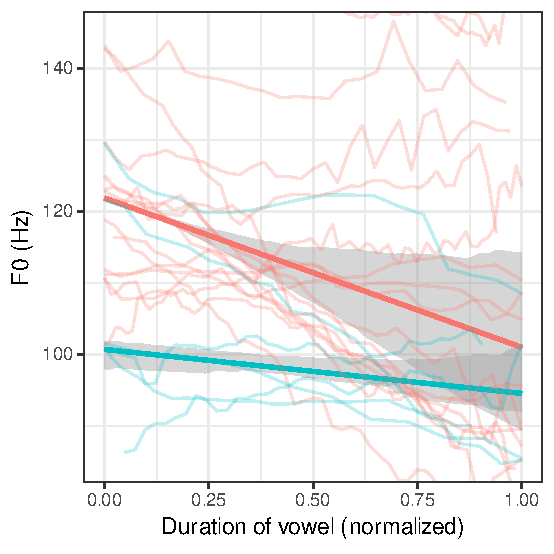
\includegraphics{figure/vowel-pitch-HL-postclause-manual-1.pdf}
\caption{Pitch trajectories of lexical H (top) and L (bottom) vowels at
the boundary for post-clause
constituents.\label{fig:vowel_pitch_HL_postclause_manual}}
\end{figure}

Finally, Figure \ref{fig:vowel_pitch_HL_uttfinal_manual} treats the
boundary correlating with the end of the utterance.

\begin{figure}
\centering
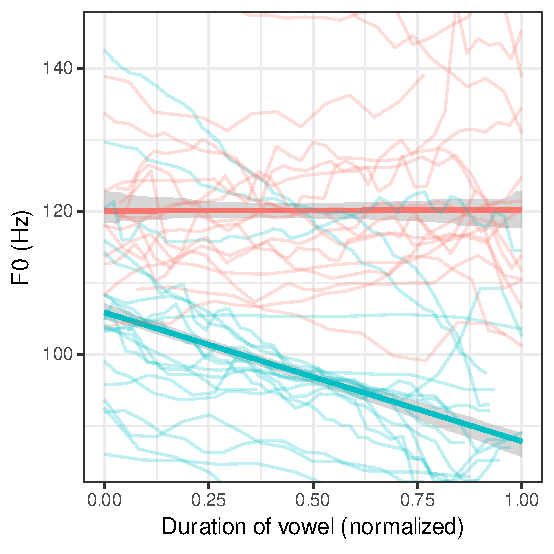
\includegraphics{figure/vowel-pitch_HL-uttfinal-manual-1.pdf}
\caption{Pitch trajectories of lexical H (top) and L (bottom) vowels at
the utterance final TBU.\label{fig:vowel_pitch_HL_uttfinal_manual}}
\end{figure}

Here, lexical H does not undergo lowering of the F0 of production over
the duration of the vowel. The F0 of production for lexical L lowers
again over the duration of the vowel, with the median line showing an
approximate lowering of 18 Hz.

\hypertarget{discussion}{%
\section{Discussion}\label{discussion}}

In Figure \ref{fig:transition_to_toneless}, we find confirmation of the
observation in \textcite{Beavon-Ham2019Tone} that H and L tone spread
are relevant processes in the tonal phonology of Saxwe, but beyond this
we see detail about how tonal spread is realized. When we examine the
transition of lexical H to an underlying Ø vowel in Figure
\ref{fig:transition_to_toneless}, we see that the vowel which is
underlyingly Ø does not simply match the F0 of H, but in fact the peak
of F0 production occurs on the second (underlyingly Ø) vowel of this
transition. Peak delay, as defined by \textcite{xu_fundamental_2001}, is
described as ``an F0 peak that sometimes occurs after the syllable it is
associated with either lexically or prosodically'' (p.~26). Other
definitions of peak delay may refer to the late realization of an F0
peak within the syllable to which the tone is associated
\autocite{myers_tone_1999}, but in the definition employed by Xu, the F0
peak is realized specifically after the syllable associated with that
tone. In the H→Ø transition, there is a median pitch interval of
approximately +0.6 semitones that is a statistically significant
difference from a zero pitch difference.

Furthermore, in the transition of lexical L to an underlying Ø vowel in
Figure \ref{fig:transition_to_toneless}, we see that the vowel which is
underlyingly Ø does not simply match the F0 of L, but in fact the trough
of F0 production occurs on the second (underlyingly Ø) vowel of this
transition. There is a median pitch interval of approximately -0.6
semitones in the L→Ø transition that is a statistically significant
difference from a zero pitch difference. These findings are in contrast
to the finding that there is no statistically significant pitch change
in the transition from one vowel that is underlyingly Ø to another vowel
that is underlyingly Ø.

Figure \ref{fig:downstep_transition} shows that there is a large amount
of variation in how pitch intervals are realized for particular lexical
tone transitions. This leads to some rare and surprising observations;
e.g.~L→H is occasionally realized as a pitch fall according to the
automated measurements done on this corpus.

The results shown in Figure \ref{fig:downstep_transition} are also
useful for helping to inform conclusions about whether non-automatic
downstep is a part of the implementation of tone for this speaker of
Saxwe --- although the conclusions that can be made from these results
are limited in certain respects. The Ø→!H transition is the locus where
the F0 lowering of non-automatic downstep occurs. It is at this
transition that the spreading of a previous lexical H across a non-zero
number of toneless vowels is stopped and we then have adjacent H tones
on the tonal tier---creating a violation of the Obligatory Contour
Principle.\footnote{As noted earlier, the !H notation is used for this
  specific context in which a lexical H is preceded by a lexical H and
  an intervening non-zero number of toneless vowels (in that order).}

As a result of this violation, we observe a lowering of pitch in this
Ø→!H transition at a median interval of approximately -2 semitones. This
is compared to the H→L transition which is also a lowering of pitch, but
which has a median interval of approximately -4 semitones. The
interquartile range and the 95\% confidence intervals of the Ø→!H pitch
change both appear relatively small compared to those of either of the
H→L and L→H transitions in Figure \ref{fig:downstep_transition}. There
are a few possible interpretations for this observation. Perhaps the
simplest is the difference in the number of samples, as there are 101
samples of Ø→!H but only 54 samples of H→L. However the L→H transition,
which has 104 samples, does have a similar wide distribution. Another
possibility is that the Ø→!H transition, being the immediate locus of
non-automatic downstep, is a carefully controlled pitch change intended
to be clearly distinguished from the H→L transition. The other
interpretation is that it is not the Ø→!H transition that is implemented
with relative precision, but it is rather the H→L transition which is
implemented with a relative lack of precision, the H being subject to
anticipatory raising effects before L \autocite{laniran_downstep_2003}.
It is not in the scope of this study to determine which of these
interpretations is the correct one.

We turn now to a discussion of the interplay in Saxwe between lexical
tone and boundary tone. In Figure
\ref{fig:vowel_sequences_and_medial_boundaries_manual}, we find evidence
of pitch resetting within the utterance after crossing an IP boundary
which is internal within the utterance (correlating with either fronted
constituents or post-clause constituents). When two vowels having
identical lexical tones immediately precede these utterance-medial IP
boundaries, the second vowel is produced on average at a F0 which is
lower than the first. However, when two vowels having identical lexical
tones are found on either side of these utterance-medial boundaries, the
second vowel is produced on average at a F0 which is higher than the
first. This can be identified as pitch resetting, which is described in
\textcite{kugler_tone_2017} for Akan. In Akan, pitch resetting occurs at
the IP boundary occurring after fronted constituents and in complex
declarative sentences.\footnote{The definition of the latter category
  overlaps with our definition of the IP boundary correlating with
  post-clause constituents, except that in this study we include
  coordination in the category of IP boundaries correlated with
  post-clause constituents.} Kügler describes pitch resetting as a
raising of the pitch register that signals embedding of one intonational
phrase within another.

In Figure \ref{fig:vowel_sequences_and_medial_boundaries_manual}, we
compare the difference in F0 realization between \emph{all} instances of
consecutive identical lexical tones which immediately precede or cross
an utterance-medial IP boundary. We do not examine individually the
realization of pitch resetting for each lexical tone; e.g.~for H→H or
L→L. This enables us to have more statistically significant findings
regarding pitch resetting in this corpus. The disadvantage of this
choice is that we cannot investigate whether L and H show different
resetting patterns.

When we narrow our examination to the pitch \emph{trajectory} of the
vowels immediately preceding the IP boundary correlated with fronted
constituents, we see clear evidence of accommodation between lexical
tone and boundary tone. According to definitions given in
\textcite{hyman_tonal_2011}, accommodation is seen when F0 patterns
include observations attributable to both the lexical tone and the
boundary tone. They explain that this may be observed solely on the
final syllable of the utterance or it may be observed over multiple
syllables in the utterance.

We see in Figure \ref{fig:vowel_pitch_HL_fronted_manual} that initially
in the duration of the vowel, the pitch trajectories for H and L are
distinct, and by the end of duration of the vowel, there is complete
neutralization between the two lexical tones with regard to F0
production. Both lexical tone and boundary tone have an effect on the
vowel at this boundary; initially, lexical tone exerts a greater
influence and by the end, boundary tone exerts a greater
influence.\footnote{Note that the evidence from this study does not
  support the analysis in \textcite{Beavon-Ham2019Tone} proposing a LH\%
  boundary tone for fronted constituents (labeled as topics in that
  study).}

This neutralization is seen to a lesser degree at the boundary
correlated with post-clause constituents. In Figure
\ref{fig:vowel_pitch_HL_postclause_manual}, there is not the same
unequivocal overlap of pitch trajectories of H and L at the end of the
duration of the vowel. We see again a lowering of the pitch trajectory
of lexical H over the duration of the vowel when looking at the solid
line representing median values of the data. However, the lines
depicting individual pitch trajectories raise the question of whether
there are two trends happening, one involving the lowering of lexical H
and the other involving a stable production of pitch of lexical H at
this boundary.

These observations could be the result of an unhelpful conflation of two
types of phonologically distinctive IPs within our single category of
the IP for post-clause constituents. This is a topic that needs to be
investigated further. For example, further investigation could entail
separating out coordinate clauses from dependent clauses which follow
the main clause. The risk of doing this with the corpus used in this
study is that this would likely yield statistically inconclusive results
(i.e.~estimating an average trajectory from a handful of samples). We
can therefore only tentatively label a subset of the post-clause IP
boundary utterances as having L tone associated with them, represented
as L\%. It is clear that at least some of the IPs show accommodation
between lexical H tone and a L\% boundary. However, further
investigation is necessary to better define the type of IP this L\%
boundary is associated with.

Now we can contrast all of the findings related to utterance-medial
boundaries with Figure \ref{fig:vowel_pitch_HL_uttfinal_manual} which
shows pitch trajectories for lexical H and L at an utterance-final
boundary. Here, H is unaffected by being at an utterance-final boundary.
The lowering of the F0 of production of lexical L shows to be at a
steeper downward slope than that seen for lexical L in the absence of a
boundary, seen in Figure \ref{fig:vowel_pitch_HL_noboundary_manual}. The
difference that can be observed is that between a median lowering of
approximately 8 Hz over the duration of the L vowel in the absence of a
boundary, and a median lowering of approximately 18 Hz over the duration
of the L vowel at the utterance-final IP boundary. This observation
seems to indicate the presence of an utterance-final L\% boundary tone.

What is the relationship between lexical H and the utterance-final L\%
boundary, if there is one? We conclude from the observations of lexical
H that either: 1) there is no utterance-final L\% boundary (despite the
slope of lowering of lexical L), or 2) there is an utterance-final L\%
boundary observable through the lowering of L and other means, but which
has a relation of avoidance with lexical H such that H avoids influence
from the L\% boundary tone.\footnote{An utterance-final L\% boundary is
  used in \textcite{Beavon-Ham2019Tone} to explain the HL surface
  realization that is seen when the lexical sequence HØ occurs finally.
  We see a single instance of this HL surface realization in Figure
  \ref{fig:pc1} on the final lexical HØ sequence. The data used in this
  study did not include enough occurrences of utterance-final lexical
  sequences of HØ (or LØ) to allow for a statistically significant study
  of this particular context of interaction between lexical and boundary
  tone. Further research on this topic would yield a more complete
  understanding of the final L\% boundary in Saxwe.}
\textcite{hyman_tonal_2011} speak of ``incomplete avoidance'', in which
one or more lexical tones avoid the influence of boundary tone. This
utterance-final boundary would be the only IP boundary where lexical H
tone is impervious to the influence of boundary tone.

The L\% boundary for fronted constituents has a relationship of
accommodation with lexical H and L. In contrast with this, the
utterance-final boundary appears to have a relationship of incomplete
avoidance, in which lexical H avoids the influence of the boundary. If
we consider the utterance-final position to be the default for IP
boundaries, we can see that the more significant pitch changes coincide
with the more marked locations for an IP boundary.

We now turn to some interesting findings regarding the pitch
trajectories for the F0 production of lexical L. It is not uncommon in
descriptions of African tone systems to speak of a falling L which is
observed before a pause in contrast with non-falling L realized
phrase-medially \autocite[pp.~175,230]{snider_tone_2018}. In every pitch
trajectory of lexical L that we examine in this study, L has a falling
pitch trajectory. To our knowledge, this is an observation not made in
any previous description of the implementation of tone in Gbe languages.
This falling pitch trajectory is seen in contexts where lexical L is at
an IP boundary as well as in contexts where no IP boundary is present.
The slope of lowering differs according to the context, seen as: 1) a
median lowering of approximately 8 Hz over the duration of the L vowel
in the absence of a boundary, 2) a median lowering of approximately 33
Hz over the duration of the L vowel at the IP boundary of a fronted
constituent, and 3) a median lowering of approximately 18 Hz over the
duration of the L vowel at the utterance-final IP boundary.

The steepest falling pitch of lexical L is therefore at the IP boundary
of a fronted constituent, perhaps because this combination of lexical L
with a L\% boundary occurs early in the utterance before declination has
brought the overall level of production of F0 down, thereby compressing
the possible range of pitch production. The next steepest pitch slope of
lexical L is at the utterance-final IP boundary. Utterance-finally,
lexical L has a median 18 Hz fall over the duration of the vowel as
compared to a median 8 Hz fall over the duration of the vowel in the
absence of any boundary. From the data we have obtained in this study,
this is the clearest indicator of the possible presence of an
utterance-final L\% boundary in Saxwe. Further exploration of this
question would treat other factors that might confirm the presence of an
utterance-final L\% boundary.

This study has been undertaken in part with the intention of assessing
the benefits and limitations of applying automatic alignment tools to a
corpus to study tone. There are certain limitations inherent in this
type of corpus-based study.

In unprepared texts such as these, it is difficult to assess any
measurement of the lowering that might be due to declination, as it is
relatively rare to have a long sequence of identical lexical tones in a
naturally occurring context.

Moreover, if one attempts to examine transitions over sequences of more
than two adjacent vowels, one does not find enough data to be able to
confidently draw conclusions. In this study, this means for example that
we are unable to address the question of whether the register lowering
effect of non-automatic downstep endures over the entirety of the
utterance.

Certain complexities are introduced by a corpus of texts that are absent
in more controlled elicitation sessions. Because of the large number of
lexical items in the corpus, there is a risk of error in the assignment
of some of the lexical tones. Moreover, there can be an element of
personal bias in attempting to identify pauses and lengthening in the
stream of speech that signal IP boundaries. In natural speech, syntactic
structures are not processed or agreed upon prior to speech production.
Because of this, issues like run-on utterances, retakes, and the
speaker's levels of energy can blur intonational cues that might
otherwise be realized with more intention and differentiation in a
controlled setting.

One advantage of this approach is the possibility of obtaining
statistically significant validation of observations made in an elicited
environment. Another advantage is the reverse: the possibility of
discovering that the preponderance of evidence in a corpus may not
validate observations made through observations of individual elicited
utterances. One also has the possibility of investigating in an
automated way pitch phenomena within a single vowel or across sequences
of adjacent vowels.

One can imagine a number of applications for this type of corpus-based
analysis of tone in texts. One possibility would be to examine other
phonetic correlates of IP boundaries apart from pitch. This could
include examining for potential devoicing and lengthening of a vowel
located at the various IP boundaries examined in this study.

Finally, looking more broadly than purely academic interests, one can
imagine text-to-speech applications for the type of study done here. As
text-to-speech becomes a possibility for under-resourced languages, one
of the things that would make speech outputs sound natural is a detailed
understanding of tone production gained from a variety of corpora
obtained from a variety of speakers.

\hypertarget{acknowledgements}{%
\section{Acknowledgements}\label{acknowledgements}}

The research for this paper was done as part of the SIL International
Pike Scholars program. We are grateful to André Taïve for his many hours
of patient work in providing texts and correcting transcriptions. Joshua
Ham, Matthew Kempton, and two anonymous reviewers provided helpful
feedback leading to improvements on earlier versions of this paper; we
are grateful for their time and attention to detail.

\printbibliography[title=References]

\end{document}
